\documentclass{article}
\usepackage{amsmath, sfmath, multicol, tkz-euclide, array, enumerate, tcolorbox, tabularray}
\renewcommand{\familydefault}{\sfdefault}
\setlength{\parindent}{0cm}
\pagestyle{empty}
\usepackage[left=1in, top=0.5in, right=1in, bottom=0.5in]{geometry}
\tikzset{>=stealth, label style/.append style={font=\footnotesize}}
\tcbset{colback=white}

\newcounter{example}[section]
\newenvironment{example}[1][]{\refstepcounter{example}\par\medskip
   {\color{red}\textbf{Example~\theexample. #1}}}{\medskip}

\begin{document}

\section*{Properties of Rectangles, Rhombi, and Squares}

\begin{tcolorbox}[colframe=orange!70!white, coltitle=black, title=\textbf{Today I Can}]
\begin{enumerate}
    \item Define and classify special types of parallelograms.
    \item Use properties of diagonals of rhombi and rectangles.
\end{enumerate}
\end{tcolorbox}
\bigskip 

\begin{tcolorbox}[colframe=black!20!white, opacitybacktitle=0.1, coltitle=black, title=\textbf{Rhombus}]
A parallelogram with all sides congruent. \newline 

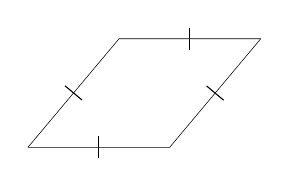
\begin{tikzpicture}[scale=0.6]
\tkzDefPoints{0/0/A, 3/0/B}
\tkzDefShiftPoint[A](50:3){C}
\tkzDefShiftPoint[B](50:3){D}
\tkzDrawPolygon(A,B,D,C)
\tkzMarkSegments[mark=|](A,B B,D C,D C,A)
\end{tikzpicture}
\end{tcolorbox}

\begin{example}
Find the measure of each numbered angle in each rhombus.
\begin{multicols}{2}
\begin{enumerate}[(a)]
    \item \mbox{}
    \item \mbox{} 
\end{enumerate}
\end{multicols}
\begin{minipage}{0.5\textwidth}
    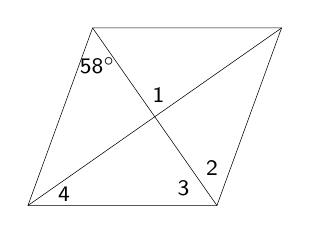
\begin{tikzpicture}[scale=0.8]
    \tkzDefPoints{0/0/A, 3/0/B}
    \tkzDefShiftPoint[A](70:3){D}
    \tkzDefShiftPoint[B](70:3){C}
    \tkzDrawPolygon(A,B,C,D)
    \tkzDrawSegments(A,C B,D)
    \tkzInterLL(A,C)(B,D)
    \tkzGetPoint{E}
    \tkzLabelAngle[pos=0.6](A,D,B){\footnotesize $58^\circ$}
    \tkzLabelAngle[pos=0.35](B,E,A){\footnotesize 1}
    \tkzLabelAngle[pos=0.6](B,A,E){\footnotesize 4}
    \tkzLabelAngle[pos=0.6](C,B,E){\footnotesize 2}
    \tkzLabelAngle[pos=0.6](E,B,A){\footnotesize 3}
    \end{tikzpicture}
\end{minipage}
\begin{minipage}{0.4\textwidth}
    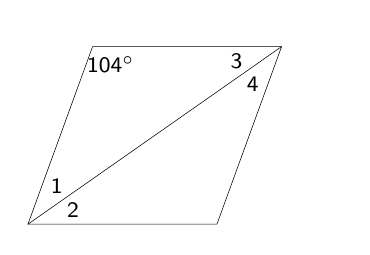
\begin{tikzpicture}[scale=0.8]
    \tkzDefPoints{0/0/A, 3/0/B}
    \tkzDefShiftPoint[A](70:3){D}
    \tkzDefShiftPoint[B](70:3){C}
    \tkzDrawPolygon(A,B,C,D)
    \tkzDrawSegment(A,C)
    \tkzLabelAngle[pos=0.5, yshift=0.1cm](A,D,C){\footnotesize $104^\circ$}
    \tkzLabelAngle[pos=0.75](C,A,D){\footnotesize 1}
    \tkzLabelAngle[pos=0.75](B,A,C){\footnotesize 2}
    \tkzLabelAngle[pos=-0.75](A,C,D){\footnotesize 3}
    \tkzLabelAngle[pos=0.75](A,C,B){\footnotesize 4}
    \end{tikzpicture}
\end{minipage}
\end{example}

\vfill 

\begin{tcolorbox}[colframe=black!20!white, opacitybacktitle=0.1, coltitle=black, title=\textbf{Rectangle}]
A parallelogram with 4 right angles. \newline 

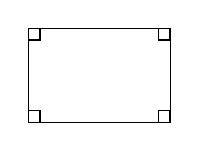
\begin{tikzpicture}[scale=0.6]
\tkzDefPoints{0/0/A, 3/0/B, 3/2/C, 0/2/D}
\tkzDrawPolygon(A,B,C,D)
\tkzMarkRightAngles(B,A,D C,B,A B,C,D C,D,A)
\end{tikzpicture}
\end{tcolorbox}

\begin{example}
Find the length of the diagonal in each rectangle.
\begin{multicols}{2}
\begin{enumerate}[(a)]
    \item $SF=2x+15 \text{ and } RB=5x-12$
    \item $LN=4x-17 \text{ and } MO=2x+13$
\end{enumerate}
\end{multicols}
\begin{minipage}{0.5\textwidth}
    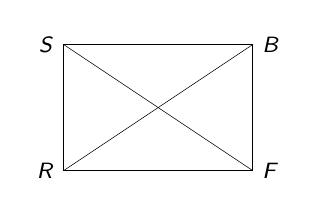
\begin{tikzpicture}[scale=0.8]
    \tkzDefPoints{0/0/R, 3/0/F, 3/2/B, 0/2/S}
    \tkzDrawPolygon(R,F,B,S)
    \tkzDrawSegments(R,B F,S)
    \tkzLabelPoints[left](R,S)
    \tkzLabelPoints[right](B,F)
    \end{tikzpicture}
\end{minipage}
\begin{minipage}{0.4\textwidth}
    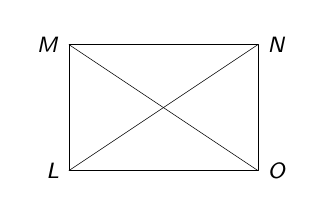
\begin{tikzpicture}[scale=0.8]
    \tkzDefPoints{0/0/L, 3/0/O, 3/2/N, 0/2/M}
    \tkzDrawPolygon(L,O,N,M)
    \tkzDrawSegments(L,N O,M)
    \tkzLabelPoints[left](L,M)
    \tkzLabelPoints[right](O,N)
    \end{tikzpicture}
\end{minipage}
\end{example}

\vfill 
\newpage 

\begin{tcolorbox}[colframe=black!20!white, opacitybacktitle=0.1, coltitle=black, title=\textbf{Square}]
A parallelogram that is \emph{both} a rectangle and a rhombus. \newline 

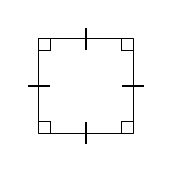
\begin{tikzpicture}[scale=0.6]
\tkzDefPoints{0/0/A, 2/0/B, 2/2/C, 0/2/D}
\tkzDrawPolygon(A,B,C,D)
\tkzMarkRightAngles(B,A,D C,B,A B,C,D C,D,A)
\tkzMarkSegments[mark=|](A,B B,C C,D D,A)
\end{tikzpicture}
\end{tcolorbox}

\begin{example}
Classify each of the following as either a rectangle, rhombus, or square.
\begin{enumerate}[(a)]
    \item $K(4, \, 8), \, L(0, \, 9), \, M(-2, \, 1), \, N(2, \, 0)$ \newline\\

    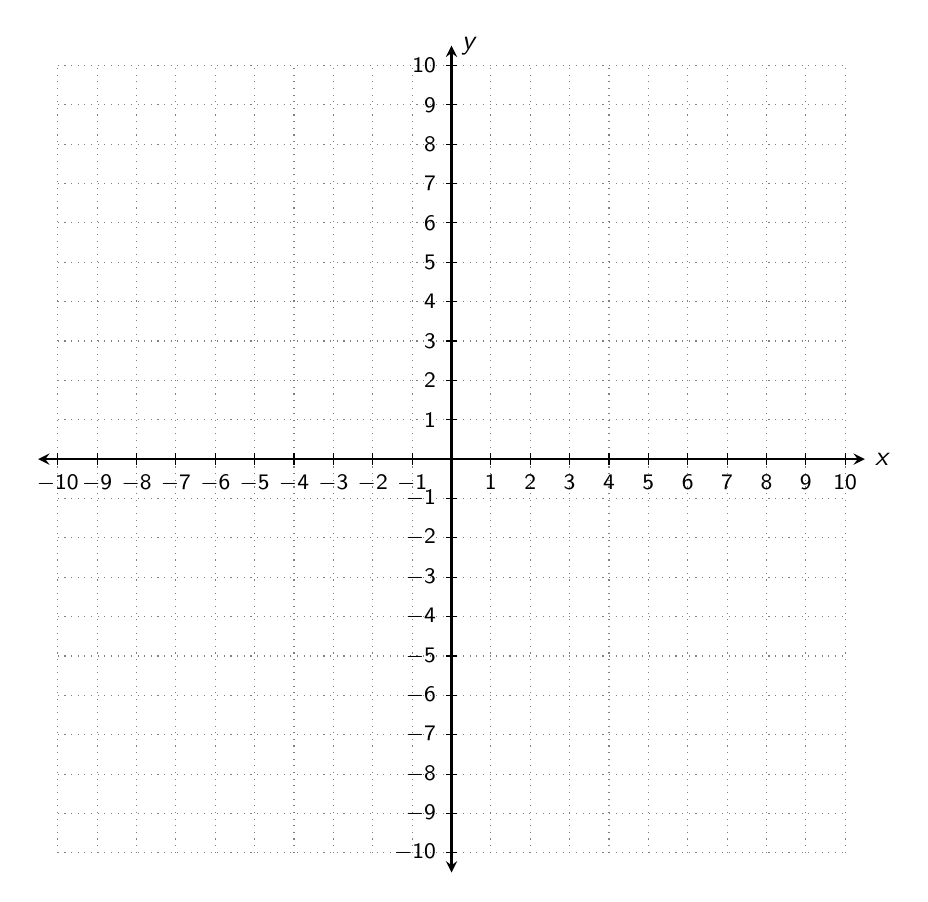
\begin{tikzpicture}[scale=0.5]
    \draw [gray, dotted] (-10,-10) grid (10,10);
    \draw [<->, thick] (-10.5,0) -- (10.5,0) node [right] {$x$};
    \foreach \x in {-10,...,-1,,1,...,10}
    \draw (\x, 0.15) -- (\x, -0.15) node [below] {\footnotesize $\x$};
    \draw [<->, thick] (0,-10.5) -- (0,10.5) node [right] {$y$};
    \foreach \y in {-10,...,-1,,1,...,10}
    \draw (0.15,\y) -- (-0.15, \y) node [left] {\footnotesize $\y$};
    \end{tikzpicture}

    \vfill 
    
    \item $A(-5, \, 0), \, B(2, \, -6), \, C(8, \, 1), \, D(1, \, 7)$   \newline\\

    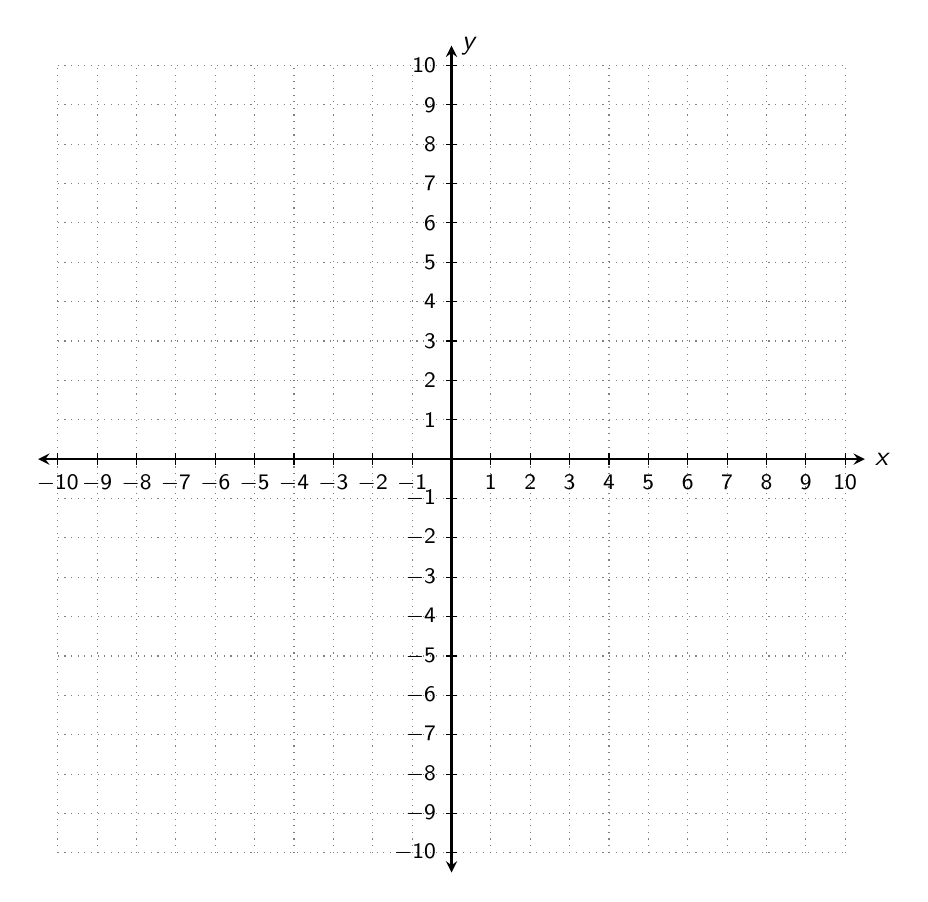
\begin{tikzpicture}[scale=0.5]
    \draw [gray, dotted] (-10,-10) grid (10,10);
    \draw [<->, thick] (-10.5,0) -- (10.5,0) node [right] {$x$};
    \foreach \x in {-10,...,-1,,1,...,10}
    \draw (\x, 0.15) -- (\x, -0.15) node [below] {\footnotesize $\x$};
    \draw [<->, thick] (0,-10.5) -- (0,10.5) node [right] {$y$};
    \foreach \y in {-10,...,-1,,1,...,10}
    \draw (0.15,\y) -- (-0.15, \y) node [left] {\footnotesize $\y$};
    \end{tikzpicture}
\end{enumerate}
\end{example}

\end{document}
